\section{Regras}

\begin{figure}[H]
  \centering
  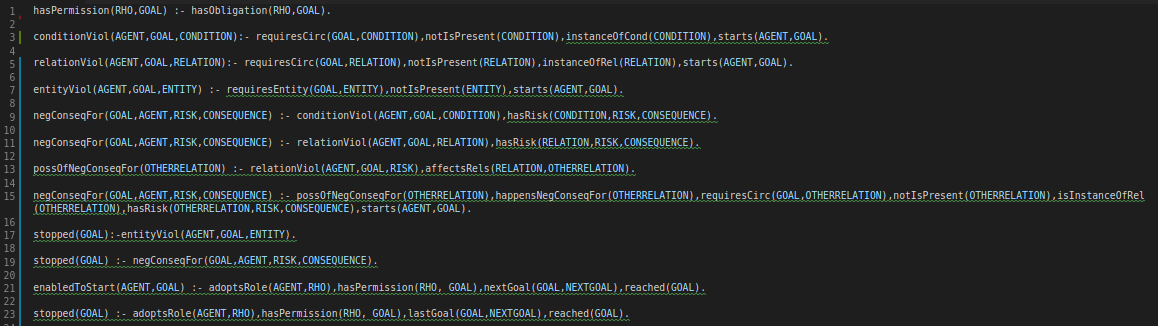
\includegraphics[width=1.1\linewidth]{figure/rules} 
  \caption{Regras}
  \label{atividiagram2}
\end{figure}



\section{Raciocínio 1}

adoptsRole(agente4,executor2).

hasObligation(executor2,g1).

requiresCirc(g1,relPanoGlicerina).

instanceOfRel(relPanoGlicerina). 

starts(agente4,g1).

notIsPresent(relPanoGlicerina).

affectsRels(relPanoGlicerina,relBastaoGarraCondutor).

affectsRels(relPanoGlicerina,relCordaEstropo).

affectsRels(relPanoGlicerina,relChaveCatracaParafuso).

affectsRels(relPanoGlicerina,relParafusoConector).

affectsRels(relPanoGlicerina,relSoqueteParafuso).

affectsRels(relPanoGlicerina,relAgente4Corda).

affectsRels(relPanoGlicerina,relEstropoCorda).


\section{Raciocínio 2}

adoptsRole(agente2,executor1). 

adoptsRole(agente3,executor1).	 	

adoptsRole(agente4,executor2).	 

hasObligation(executor1,g1).

hasObligation(executor2,g1).

starts(agente2,g1). 

starts(agente3,g1).	 	

starts(agente4,g1).

requiresEntity(g1,pano).		

notIsPresent(pano).

\section{Raciocínio 3}


adoptsRole(agente5,executor3).

hasObligation(executor3,g11).	

starts(agente5,g11).

requiresCirc(g11,umidade70).

instanceOfCond(umidade70).

notIsPresent(umidade70).

hasRisk(umidade70,eletrocutado,morte).

\section{Raciocínio 4}

adoptsRole(agente4,executor2).

hasObligation(executor4,g15).	

starts(agente4,g15).

requiresCirc(g15,relChaveCatracaParafuso).

instanceOfRel(relChaveCatracaParafuso).	

notIsPresent(relChaveCatracaParafuso).

hasRisk(relChaveCatracaParafuso,eletrocutado,morte).

\section{Raciocínio 5}

requiresCirc(g19,relParafusoConector).

hasObligation(executor3,g19).

hasObligation(executor4,g19).

hasObligation(executor5,g19).

starts(agente5,g19).

starts(agente6,g19).

starts(agente7,g19).

adoptsRole(agente5,executor3).

adoptsRole(agente6,executor4).

adoptsRole(agente7,executor5).

hasRisk(relParafusoConector,eletrocutado).

possOfNegConseqFor(relParafusoConector).

happensNegConseqFor(relParafusoConector).

instanceOfRel(relParafusoConector).

hasRisk(relParafusoConector,eletrocutado,morte).

\section{Raciocínio 6}


\begin{figure}[H]
  \centering
  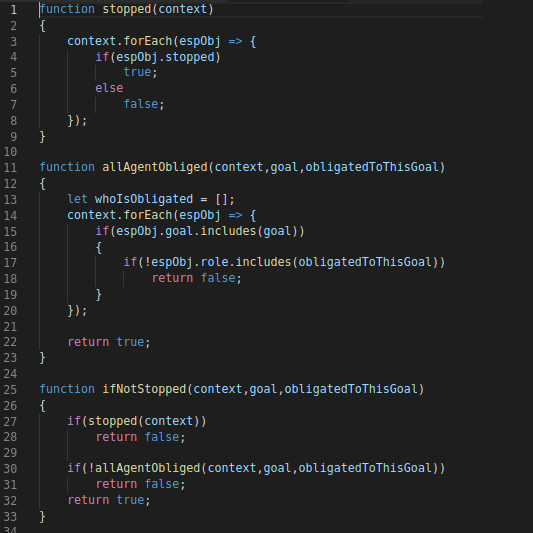
\includegraphics[width=0.8\linewidth]{figure/algjs} 
  \caption{Raciocínio 6 parte 1}
  \label{atividiagram2}
\end{figure}


\begin{figure}[H]
  \centering
  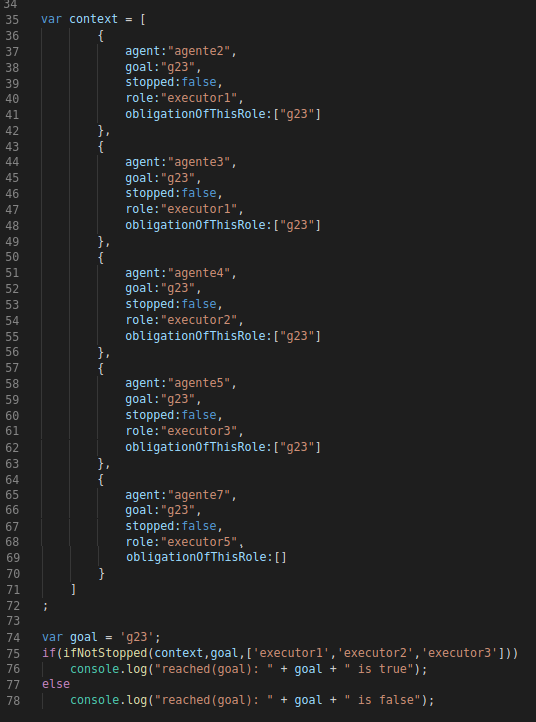
\includegraphics[width=0.8\linewidth]{figure/algjs2} 
  \caption{Raciocínio 6 parte 2}
  \label{atividiagram2}
\end{figure}
